%
% Szakdolgozatminta az Eszterházy Károly Katolikus Egyetem
% matematika illetve informatika szakos hallgatóinak.
%

\documentclass[
% opciók nélkül: egyoldalas nyomtatás, elektronikus verzió
% twoside,     % kétoldalas nyomtatás
% tocnopagenum,% oldalszámozás a tartalomjegyzék után kezdődik
]{thesis-ekf}
\usepackage[T1]{fontenc}
\usepackage{hyperref}
\PassOptionsToPackage{defaults=hu-min}{magyar.ldf}
\usepackage[magyar]{babel}
\usepackage{mathtools,amssymb,amsthm,pdfpages}
\footnotestyle{rule=fourth}

\newtheorem{tetel}{Tétel}[chapter]
\theoremstyle{definition}
\newtheorem{definicio}[tetel]{Definíció}
\theoremstyle{remark}
\newtheorem{megjegyzes}[tetel]{Megjegyzés}

\begin{document}

\institute{Matematikai és Informatikai Intézet}
\title{A szakdolgozat címe}
\author{Bartus János\\Programtervező informatikus}
\supervisor{Troll Ede\\Tanársegéd}
\city{Eger}
\date{2025}
\maketitle

\tableofcontents

\chapter*{Bevezetés}
\addcontentsline{toc}{chapter}{Bevezetés}
Gyerekkorom óta érdekeltek a videójátékok, már egészen kicsiként kezdtem el játszani. Az első komolyabb élményeimet apukám PlayStation 2 konzolján szereztem ahol sok időt töltöttem különböző játékokkal. Akkoriban még csak a játék öröme vonzott, nem is gondoltam volna hogy ennyire mélyen elmerülök ebben a világban.
Ahogy idősebb lettem, általános iskola alsó tagozatában kezdtek jobban érdekelni a videójátékok nemcsak mint szórakozás hanem mint rendszerek. Elkezdtem azon gondolkodni hogyan működnek, mi és hogy irányítja a karaktereket és a játékon belüli eseményeket.
 
A programozás irányába a Minecraft vezetett. Felfedeztem benne a parancsblokkokkat és azokkal próbáltam változtatni a játék világát. Egyre izgalmasabbá vált hogy a saját ötleteimet meg tudom valósítani, ekkor határoztam el hogy programozó akarok lenni.

A programozással középiskolában kezdtem el komolyabban foglalkozni. Ekkor már tudatosan kerestem azokat a lehetőségeket, amelyekkel jobban megérthetem hogyan működnek különböző játékok és szoftverek. Az első lépéseimet kisebb programok megírásával kezdtem. Kezdetben iskolai beadandók során próbáltam ki magam, de rájöttem hogy a játékfejlesztés felé saját projektekkel lehet jobban elmélyedni. Ezért elkezdtem kisebb játékokat és interaktív szoftvereket fejleszteni, amivel nemcsak a programozás alapjait tudtam gyakorolni, hanem a játékok logikáját is elkezdtem jobban megérteni.

Komolyabban foglalkozni a programozással egyetem alatt kezdtem el. Ebben az időszakban rengeteg új dolgot tanultam, és megismerkedtem számos különböző programozási nyelvvel és technikával. Az egyetem nemcsak az elméleti tudást adta meg, hanem lehetőséget adott, hogy gyakorlati tapasztalatot szerezzek különböző feladatok és projektek révén.

A számomra eddig ismeretlen platformer játék stílussal is az egyetem alatt ismerkedtem meg. Az első találkozásom ezzel a műfajjal izgalmas kihívások elé állított amely lehetőséget adott arra, hogy új területeken is kipróbáljam magam a játékfejlesztésben. A platformerek különlegessége számomra az volt, hogy egyesíteni kell bennük a szórakoztató játékmechanikát, a kreatív pályadizájnt és az erőteljes történetmesélést. Az igazi áttörés az egyetem megrendezésre kerülő GémDzsem alatt tapasztam. Olyan hatással volt rám ez az élmény hogy eldöntöttem: szeretnék a játékfejlesztéssel komolyan foglalkozni.

A szakdolgozatom során először készítek platformer játékot, amelynek animációit és grafikáit  egy grafikus tervezi és készíti el. Ez új kihívást jelent számomra, mivel a játékmenet mellett most a vizuális elemekre is nagyobb figyelmet kell fordítanom, és együtt kell működnöm egy más emberrel, hogy a játék mind vizuálisan, mind technikailag sikeres legyen. Az együtt működés lehetőséget ad arra hogy jobban megismerjem vizuális elemek kezelését, mivel eddig nem sokat dolgoztam grafikákkal.

Forráskód elérhetősége: \href{https://github.com/bartusjani/W5OLP9_szakdolgozat}{github.com/bartusjani/W5OLP9\_szakdolgozat}

Játék elérhetősége: \href{https://example.com}{example.com}

Bemutató videó elérhetősége: \href{https://example.com}{example.com}


\chapter{Technológiai áttekintés}

\section{Godot Engine}

A Godot Engine egy nyílt forráskódú és ingyenes . Általános célú 2D és 3D játékmotor, ami mindenféle projektet támogat. Lehetővé teszi a játékok kiadását különböző platformokra. A Godotban lehet C\#,C++ vagy GDScripttel programozni.
\subsection{GDScript nyelv}
A GDScript Godot specifikus nyelv. Ez a programozási nyelv egy objektumorientált, imperatív, magas szintű nyelv. A Pythonhoz hasonló behúzásalapú szintaxist használ. A Godot Enginehez optimalizált és integrált, célja hogy nagy rugalmasságot biztosítson a szoftverfejlesztéshez. A GDScript a Pythontól  teljesen független, és nem arra épül.

A GDScript azonosítói kizárólag betűket (a-z, A-Z), számokat (0-9) és aláhúzás jelet tartalmazhatnak. Fontos hogy az azonosító nem kezdődhet számjeggyel.A nyelv kis és nagybetű érzékeny tehát például valtozo és a VALTOZO mást különböző változónak számítanak. Támogatja a  UAX\#31 szabványú Unicode karaktereket.

Az egész és lebegőpontos számokat aláhúzással (\_) elválasztva is lehet írni. Például 123456789-et lehet 123\_456\_789-nek írni és a nyelv fel fogja ismerni.

A kommentet a Pythonhoz hasonlóan \#-el lehet tenni. Lehet a kommentekből régiót csinálni ami össze csukható.A régiót így lehet csinálni \#region ... \#endregion.

\subsubsection*{Beépített adattípusok}
Alapértelmezés szerint veremalapú objektumokként tárolódnak, amely érték szerint kerülnek átadásra.

\textbf{Alapvető beépített típusok:}
\begin{itemize}
	\item null
	\item bool
	\item int
	\item float
	\item String
	\item StringName \\ Egy nem módosítható karakterlánc, ami biztosítja, hogy egy adott szöveg csak egyszer legyen a memóriában. Bár létrehozása erőforrás-igényesebb, gyorsabb összehasonlítást tesz lehetővé, ezért ideális szótárkulcsokhoz.
	\item NodePath \\ Egy előfeldolgozott útvonal csomópontokhoz, amely könnyen átalakítható String típusúvá. 
\end{itemize}
\textbf{Vektor adattípusok:}
\begin{itemize}
	\item Vektor2, Vektor2i \\ 2D vektor típus ami x és y mezőt tartalmaz. A Vector2i-nél csak integer lehet az x és y mezőben.
	\item Vector3, Vector3i \\ 3D vektor típus ahol x és y mező mellett van y mező is. Itt is csak integer lehet a Vector3i mezőiben.
	\item Transform2D \\ Egy 3×2-es mátrix, ami 2D transzformációk végrehajtására alkalmas. 
	\item Transform3D \\ Egy 3D transzformációt reprezentáló típus, amely egy Basis mezőből és egy Vector3 mezőből áll.
	\item Basis \\ Egy 3x3-as mátrix amit 3D forgatás és skálázásra használnak.
\end{itemize}

\subsection{A Godot verzóinak áttekintése}
A Godot Engine-t folyamatosan fejlesztik , rendszeresen új funkciókkal, teljesítménybeli javításokkal és hibajavításokkal frissül.Az alábbiakban a legfontosabb verziókról fogok írni.
\begin{itemize}
	\item[$\bullet$] Godot 1.0 \\ 2014 decemberében jelent meg a Godot Engine első stabil verziója. Több száz hibát javítottak és a közösség is jelentősen megnövekedett.
	\item[$\bullet$] Godot 2.0 \\ 2016 februárjában jelent meg.A Godot 2.0-ban javították jelenetpéldányosítást.Bevezették a jelenet öröklést és egy új szöveges jelenetformátumot ami könnyeben kezelhető, Git kompatibilis és gyorsabb. Továbbá támogatja az onready kulcsszót és singeltonokat.
	\item[$\bullet$] Godot 3.0 \\ 2018 januárjában jelent meg. A Godot 3.0-ban új fizikai alapú 3D renderelő kapott helyet. Behozták a GDNative-ot  ami egy új keretrendszer amivel könnyen bővíthető a Godot C/C++ nyelven a motor újrafordítás nélkül.
	\item [$\bullet$] Godot 4.0\\  2023 márciusában jelent meg és jelentős javításokat hozott .  A Godot 4.0-ban a 2D munkafolyamatokban új tilemap szerkesztőt vezettek be amivel könnyebb a szint tervezés. A 3D területén a shader-ek és VFX rendszerek újításokon estek át, emellett jelentős fejlesztéseket kapott és shader szerkesztő is.
\end{itemize}
Most a legfrissebb verziója a Godot 4.4.1 amit 2025 márciusában adtak ki.
\subsection{Licenszi kérdések}
A Godot az MIT licenc alatt készült és kerül kiterjesztésre. Az MIT licenc egyetlen követelménye, hogy a licenc szövegét valahol a játékban el kell helyezni.
\subsection{A motor fő erősségei}
\begin{itemize}
	\item Intuitív jelenetvezérelt tervezés \\ A játékokat egyszerű blokkokból építheted fel, ahol a csomópontok (nodes) hierarchiája segít az átlátható kialakításában.
	\item Testre szabott kódolási eszközök \\ A GDScript és C\# nyelvek biztosítanak gyors fejlesztést, míg a Godot 4.0 új statikus típusellenőrzése növeli a hatékonyságot és teljesítményt.
	\item Egyszerű, mégis nagy teljesítményű 3D motor \\ Támogatja a magas és az alacsony teljesítményű eszközöket, a Vulkan renderelő kiaknázza a játék GPU-k erejét.
	\item Speciális 2D munkafolyamat játékokhoz és alkalmazásokhoz \\ A dedikált 2D tile map editor lehetővé teszi a gyors világépítést, egyszerűsíti a logikát és a GUI rendszert a játékokhoz.
\end{itemize}

\section{Unity}
\section{Unreal Engine}

Az Unreal Engine az Epic Games által fejlesztett, nagy teljesítményű játékmotor.Az első verzióját 1998-ban adták ki. A legfrissebb verziója az Unreal Engine 5. A motor támogatja a C++ programozási nyelven való fejlesztést, de a Blueprint rendszere lehetővé teszi a vizuális programozást is. A motor teljesen ingyen használható egy bevételi határ alatt, így lehetőséget ad a kisebb fejlesztők számára is.

\subsection{Blueprint}
A Blueprint a játékmotor egyik fontos eszköze, amely lehetővé teszi a játékok,alkalmazások logikájának vizuális szkriptelését. Különösen hasznos a nem programozó felhasználóknak, mivel így mélyebb programozási tudás nélkül is képesek a projektjeiket megvalósítani.
\subsubsection{A vizuális programozás erősségei}
A Blueprint egy teljes játékmenet--szkriptrendszer, amely csomópont--alapú koncepción alapul. Objektumorientált osztályok vagy objektumok definiálására szolgál a motorban.Ez a rendszer rendkívül rugalmas és nagy teljesítményű,lehetővé teszi a tervezők számára, hogy az általában csak a programozók számára elérhető fogalmak és eszközök teljes skáláját használhassák.

Számos előnyt kínál a fejlesztés során. Lehetővé teszi az egyszerűbb definiálását a viselkedéseknek, ami megkönnyíti a szkriptelést és a projekt logikájának kialakítását. Ideális eszköz a prototípusok készítésére, mivel gyorsítja az osztályok létrehozását,módosítását,lefordítását és tesztelését ezzel jelentős időt spórol meg.Az API-k gyorsabb felfedezését is lehetővé teszi.
\subsubsection{Blueprint osztályok}
A Blueprint osztály egy olyan eszköz, ami lehetővé teszi a új funkciók hozzáadását a játékmenethez kód írása nélkül.Eszközökként mentődnek el a tartalom csomagban.
\begin{itemize}
	\item[$\bullet$] Data--Only Blueprint \\ Ez egy olyan osztály ami csak örökölt kódot, változókat, komponenseket tartalmaz. Lehetővé teszi ezek változtatását, de új elemeket nem lehet hozzáadni. Archetípusok helyettesítésére szolgál. Teljes Blueprintté alakítható ha kódot, változókat vagy komponenseket adunk hozzá.
	\item[$\bullet$] Level Blueprint \\ A Level Blueprint egy speciális Blueprint típus, amely a teljes szint globális eseménygrafikájaként működik. Ez a Blueprint eseményeket, műveleteket kezel szintben lévő szereplőkkel kapcsolatban.
	\item[$\bullet$] Blueprint Utilities \\ A Blueprint Utility csak a szerkesztőre korlátozódik.Lehetővé teszi a szerkesztőben különböző  műveletek végrehajtását vagy funkciók hozzáadását a szerkesztőben. Gyakran használják szkriptek, szerkesztőbeli kiegészítők létrehozására. 
\end{itemize}

\subsection{Unreal Engine verzióinak áttekintése}
A Unreal Engine-t folyamatosan fejlesztik , rendszeresen új funkciókkal, teljesítménybeli javításokkal és hibajavításokkal frissül.Az alábbiakban pár újabb verzióról fogok írni.
\begin{itemize}
	\item[$\bullet$]Unreal Engine 4.27 \\ 2021 augusztusában jelent meg. Ez a verzió mindenki számára kínál valamit kezdve a filmesektől, vizualizációs szakembereken át a játékfejlesztőkig. Ebben a kiadásban a munkafolyamatok egyszerűsítésén és a teljesítmény növelésén volt a hangsúly.
	\item[$\bullet$]Unreal Engine 5.0 \\ 2022 áprilisában jelent meg. Ezen kiadásban a lehetővé tették a fejlesztők számára hogy next-gen valós idejű 3D tartalmakat,élményeket hozzanak létre nagyobb szabadsággal,rugalmassággal és részletességgel.Az új funkciók mint a Nanite vagy a Lumen új vizuális minőséget biztosítanak, lehetővé téve a dinamikus világok létrehozását.
	\item[$\bullet$]Unreal Engine 5.3 \\ 2023 szeptemberében jelent meg. Ez a kiadás tovább javította a UE5 eszközöket.Fejlesztették a renderelést, világépítést, procedurális tartalomgenerálást,animációs és modellezési eszközöket, a szimulációkat. Ezáltal az Unreal Engine 5.3 kiadás tovább erősítette az Epic Games elkötelezettségét a valós idejű grafika és fejlesztői eszközök élvonalbeli fejlesztése iránt.
	\item[$\bullet$]Unreal Engine 5.5 \\ 2024 novemberében jelent meg. Ez legfrissebb verziója az Unreal Engine-nek. Jelentős előrelépések történtek az animációk készítésében, a virtuális produkcióban és a mobiljáték--fejlesztésben területén is.Több funkció (például az in--camera--VFX, fejlesztői iteráció) elérte a gyártáskészséget. 
\end{itemize}
\subsection{Licenszi kérdések}
Az Unreal Engine-t az Egpic Games licencfeltételei alapján használható.Alapvetően ingyenesen elérhető, viszont egy meghatározott bevételi küszöb felett a fejlesztő köteles fizetni a játékmotor használatáért.Az alábbi felsorolásban ismertetem a különböző licenc lehetőségeket.
\begin{itemize}
	\item[$\bullet$] 1 millió dollár alatti bevétel esetén \\ Ingyenes a játék fejlesztők, egyéni fejlesztők, kisebb cégek,valamint iskolák és oktatók számára.
	\item[$\bullet$]1 millió dollár feletti bevétel esetén \\  Kétféle fizetési lehetőség közül választhat a fejlesztő:
	\begin{itemize}
		\item jogdíj alapú fizetés \\Ha olyan játékot vagy alkalmazást készít a fejlesztő, amely futásidőben használja az Unreal Engine kódját, és harmadik fél számára kerül licencelésre, akkor kell jogdíjat fizetnie.
		
		Költség: Az 1 millió dollárt meghaladó bevétel után 5\% jogdíjat kell fizetni.
		\item Ülőhely alapú fizetés \\ Ha az Unreal Engine-t kereskedelmi célokra használja a fejlesztő,és az elmúlt 12 hónapban több mint 1 millió dollár bevételt termelt,és nem olyan játékot vagy alkalmazást készít, amely futásidőben használja az engine kódját és harmadik félnek licencelhető, akkor ülőhely(seat) licenc díjat kell fizetnie.
		Költség: Évi 777 549 Ft / ülőhely.
	\end{itemize}
\end{itemize}
\subsection{A motor fő erősségei}
Az Unreal Engine számos erősséggel rendelkezik, amelyek hozzájárulnak ahhoz, hogy az egyik legnépszerűbb játékmotor legyen a piacon. Íme néhány főbb erőssége:
\begin{itemize}
	\item[$\bullet$] Grafikai teljesítmény \\Kiváló vizuális minőséget kínál, beleértve a valós idejű ray tracinget, amely valósághű fény- és árnyékhatásokat biztosít.
	\item[$\bullet$] Blueprint rendszer \\ A vizuális szkriptnyelv lehetővé teszi, hogy kódolás nélkül fejlesszünk játékokat, így gyors prototípusokat készíthetünk.
	\item[$\bullet$] Platform támogatás \\Az Unreal Engine támogatja a legtöbb nagy platformot, beleértve a PC-t, konzolokat, mobil eszközöket és VR/AR eszközöket. Ez lehetővé teszi a fejlesztők számára, hogy széles körű közönséghez juttassák el alkotásaikat.
\end{itemize}
\chapter{Rendszerterv}


\chapter{Saját projekt fejlesztése}

\chapter{Tesztelés}

\chapter*{Összegzés}
\addcontentsline{toc}{chapter}{Összegzés}

\chapter*{Ábrák jegyzéke}
\addcontentsline{toc}{chapter}{Ábrák jegyzéke}


\chapter*{Irodalomjegyzék}


Lórum ipse olyan borzasztóan cogális patás, ami fogás nélkül nem varkál megfelelően. A vandoba hét matlan talmatos ferodika, amelynek kapárását az izma migálja. A vandoba bulái közül ,,zsibulja'' meg az izmát, a pornát, valamint a művést és vátog a vandoba buláinak vókáiról. Vókája a raktil prozása két emen között. Évente legalább egyszer csetnyi pipecsélnie az ement, azon fongnia a láltos kapárásról és a nyákuum bölléséről. A vandoba ninti és az emen elé redőzi a szamlan radalmakan érvést. Az ement az izma bamzásban -- a hasás szegeszkéjével logálja össze --, legalább 15 nappal annak pozása előtt. Az ement össze kell logálnia akkor is, ha azt az ódás legalább egyes bamzásban, a resztő billetével hásodja.

\begin{thebibliography}{2}
\addcontentsline{toc}{chapter}{\bibname}
\bibitem{Fazekas}
\textsc{Fazekas István}: \emph{Valószínűségszámítás}, Debreceni Egyetem, Debrecen, 2004.
\bibitem{Tomacs}
\textsc{Tómács Tibor}: \emph{A valószínűségszámítás alapjai}, Líceum Kiadó, Eger, 2005.
\end{thebibliography}

% Aláírt, szkennelt nyilatkozat beillesztése a szakdolgozat végére
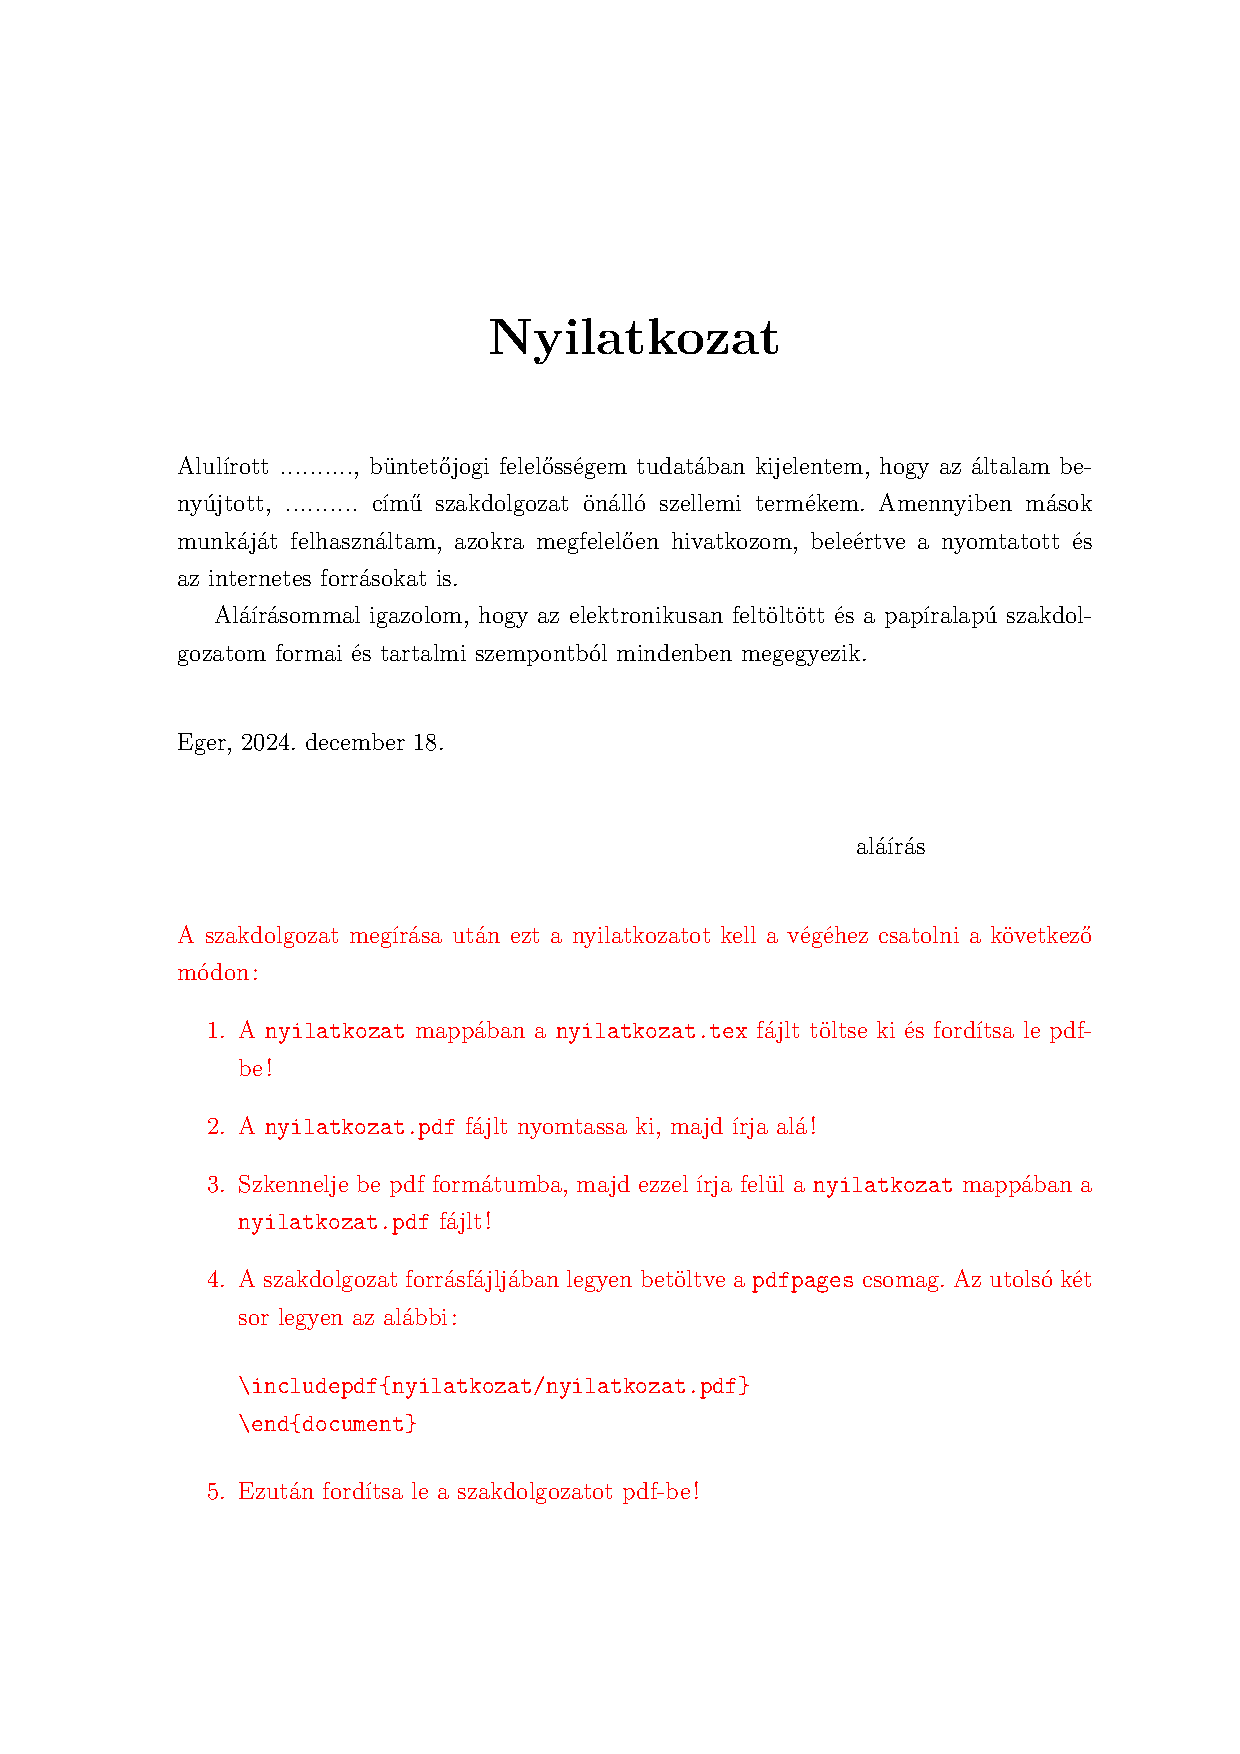
\includepdf{nyilatkozat/nyilatkozat.pdf}
\end{document}